\documentclass[11pt]{article}
%%%%%%%%%%%%%%%%%%%%%%%%%%%%
\usepackage{array, bm, geometry, epsfig, marvosym, amssymb, amsmath, float, graphics, amsthm}
\usepackage{hyperref, setspace, sectsty, alltt, fancyvrb}
\geometry{verbose, a4paper, top=0.1in, bottom=0.5in, left=0.25in, right=0.25in}
\parindent = 0.5cm
\newcommand{\code}[1]{\texttt{#1}}                      % type font
\newcommand{\hzline}[1]{\noindent\rule[0mm]{\textwidth}{#1}}

%   ---- colors ----   %
\usepackage[usenames,dvipsnames]{color}
\definecolor{lightgray}{gray}{0.75}						% gray
\definecolor{orange}{rgb}{1,0.5,0}						% orange
\definecolor{MyDarkBlue}{rgb}{0,0.08,0.45}			% dark blue
\definecolor{MyDarkGreen}{rgb}{0,0.45,0.08}			% dark green
\definecolor{purple}{rgb}{0.7,0,0.9}					% purple
\definecolor{periwinkle}{rgb}{0.8,0.8,1}				% periwinkle
\definecolor{slateblue}{rgb}{0.42, 0.35, 0.8}		% slateblue 

\let \oldv\alltt
\let \oldendv\alltt
\def \myverb{\par\topsep1pt \noindent \setbox0\vbox\bgroup\oldv}
\def \endmyverb{\oldendv\egroup\fboxsep0pt \colorbox{periwinkle}{\usebox0}\par}


\title{\textsf{Syntax for Plotting Text in R}}
\author{Stu Field}
\begin{document}

%%%%%%%%%%%%
\begin{center}
  \section*{\textsf{Syntax for Plotting Text in R}}
\end{center}
%%%%%%%%%%%%

\begin{figure}[H]
\centering
\abovecaptionskip=0pt
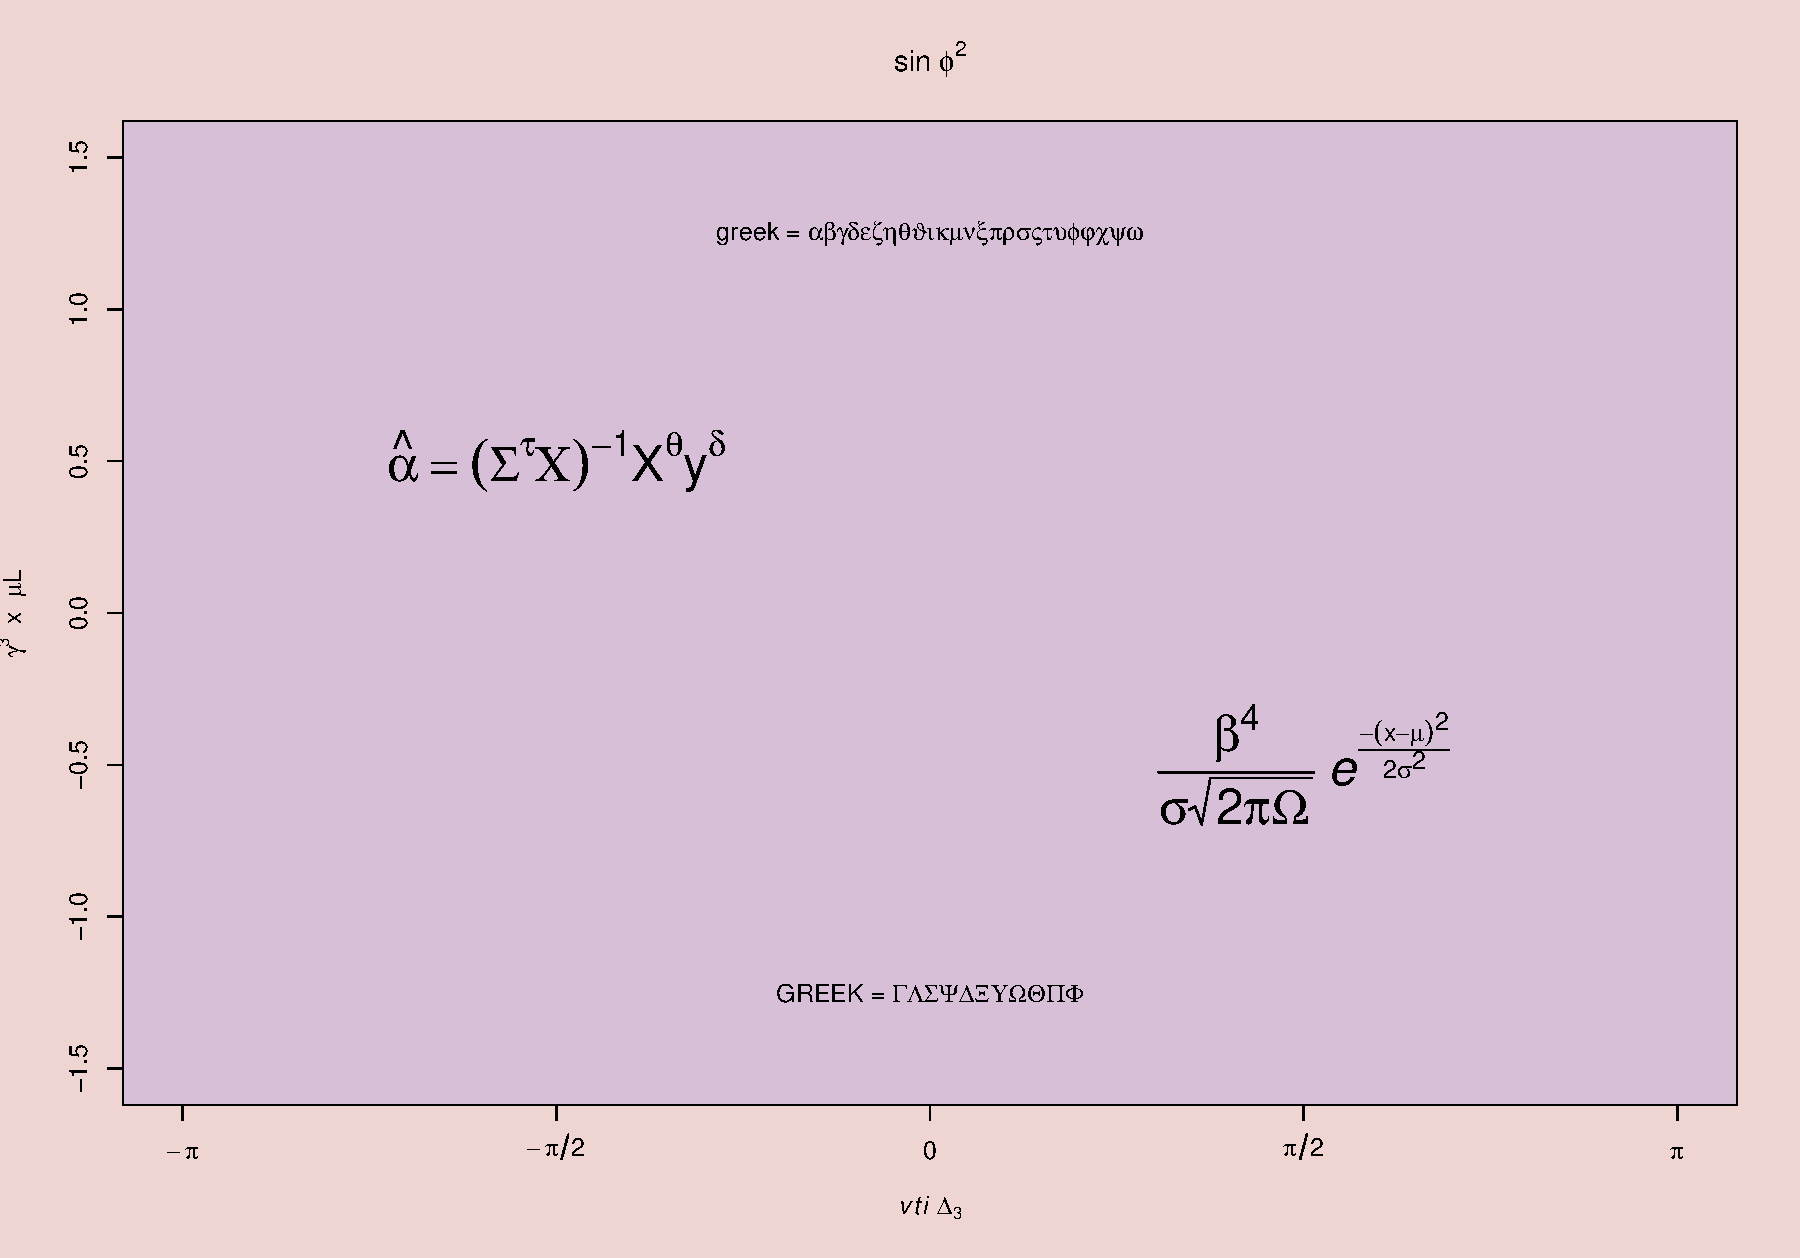
\includegraphics[width=0.95\textwidth]{fig1-symb}
\caption{Syntax examples for plotting text in \textsf{R} for axes, labels, and
  titles.}
\end{figure}

\begin{myverb}
  \input{plotSymbols.R}
\end{myverb}

\begin{figure}[H]
\centering
\abovecaptionskip=-1cm
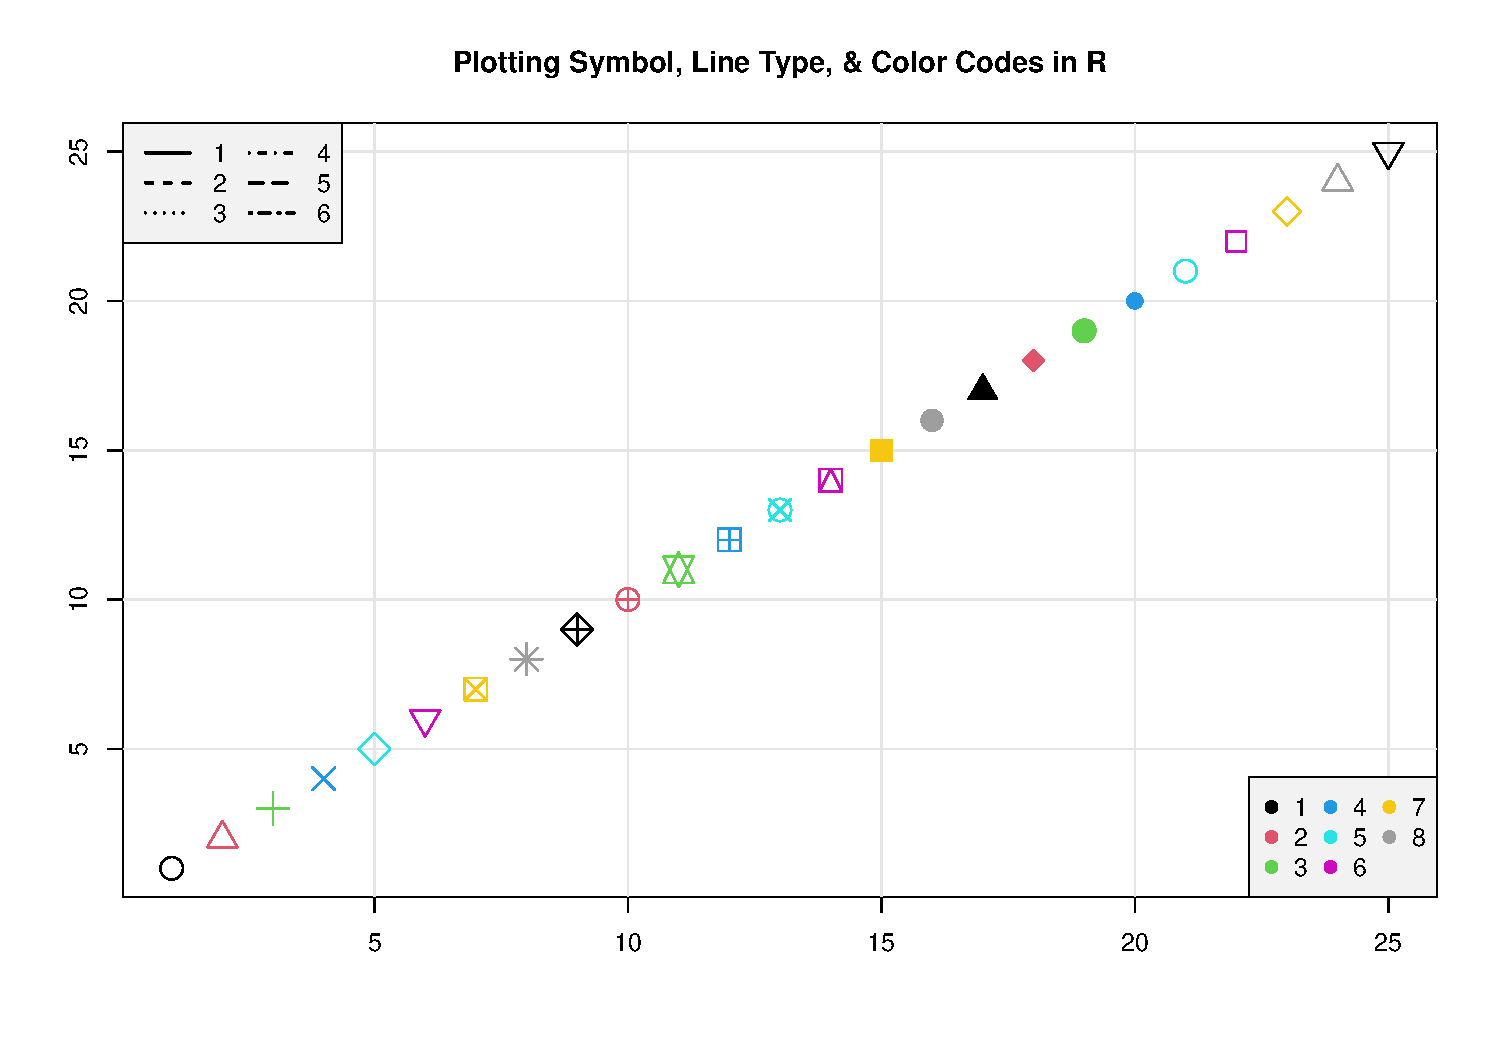
\includegraphics[width=0.99\textwidth]{fig2-pch-symb}
\caption{Basic numeric plotting codes used by \textsf{R}.
  For points, the symbols are accessed using the \code{pch=} and range
  $1 \to 25$ (some are redundant). Line types are shown in the legend, are
  accessed using the \code{lty=}, and range $1 \to 6$. Color codes range
  from $1 \to 8$ and are accessed using the
  \code{col=}. \label{fig:pchsymbols}}
\end{figure}


\begin{myverb}
  \input{plotPCHsymbols.R}
\end{myverb}

\end{document}
